\documentclass[12pt,a4paper]{report}
\hyphenpenalty=10000
\exhyphenpenalty=10000
\sloppy
\usepackage{titlesec}
\usepackage{float}
\usepackage{placeins}
\titleformat{\chapter}[display]
  {\Huge\bfseries}
  {Chapter \thechapter}
  {0pt}
  {\Huge}
  [\titlerule]
\let\cleardoublepage\clearpage
\titlespacing*{\chapter}{0pt}{-10pt}{20pt}
% Page margins
\usepackage[top=0.70in,bottom=0.80in,left=0.8in,right=0.80in]{geometry}
\titleformat{\subsubsection}
  {\normalfont\bfseries\large}
  {\thesubsubsection}
  {1em}
  {}
  \titlespacing*{\subsubsection}{0pt}{8pt}{4pt}

\titlespacing*{\section}{0pt}{10pt}{5pt}
\setlength{\parskip}{4pt}
\setlength{\parindent}{15pt}

\sloppy
% Graphics and hyperlinks
\usepackage{graphicx}
\usepackage[bookmarks,colorlinks=false]{hyperref}
\hypersetup{pdfborder={0 0 0}}

% Other packages
\usepackage[final]{pdfpages}
\usepackage{float}
\usepackage{array}
\usepackage{setspace}
\usepackage{enumerate}
\usepackage{longtable}
\usepackage{lipsum}
\usepackage[font=small,labelfont=bf]{caption}
\usepackage{pslatex}

\def\figurename{\textbf{Figure }}

% Code listing settings
\usepackage{listings}
\usepackage{xcolor}

\definecolor{dkgreen}{rgb}{0,0.6,0}
\definecolor{gray}{rgb}{0.5,0.5,0.5}
\definecolor{mauve}{rgb}{0.58,0,0.82}

\lstset{
language=Java,
basicstyle=\footnotesize,
numbers=left,
numberstyle=\tiny\color{gray},
stepnumber=1,
numbersep=5pt,
backgroundcolor=\color{white},
showspaces=false,
showstringspaces=false,
showtabs=false,
frame=single,
rulecolor=\color{black},
tabsize=2,
captionpos=b,
breaklines=true,
keywordstyle=\color{blue},
commentstyle=\color{dkgreen},
stringstyle=\color{mauve}
}

% Header and footer
\usepackage{fancyhdr}

\fancypagestyle{plain}{
\fancyfoot[L]{\emph{Department of Computer Science and Engineering (DS), SKIT, Jaipur}}
\fancyfoot[R]{\thepage}
\renewcommand{\headrulewidth}{0pt}
\renewcommand{\footrulewidth}{0.4pt}
}

\pagestyle{fancy}
\fancyhead{} 
\fancyfoot[LO,LE]{\emph{Department of Computer Science and Engineering (DS), SKIT, Jaipur}}
\fancyfoot[RO,RE]{\thepage}
\cfoot{}
\renewcommand{\headrulewidth}{0pt}
\renewcommand{\footrulewidth}{0.4pt}

% Page Border
\usepackage{pgf}
\usepackage{pgfpages}

\pgfpagesdeclarelayout{boxed}
{
\edef\pgfpageoptionborder{0pt}
}
{
\pgfpagesphysicalpageoptions{
logical pages=1
}
\pgfpageslogicalpageoptions{1}{
border code=\pgfsetlinewidth{2pt}\pgfstroke,
border shrink=\pgfpageoptionborder,
resized width=.95\pgfphysicalwidth,
resized height=.95\pgfphysicalheight,
center=\pgfpoint{.5\pgfphysicalwidth}{.5\pgfphysicalheight}
}
}
\pgfpagesuselayout{boxed}

\setlength{\parindent}{1cm}

\setcounter{tocdepth}{3}
\setcounter{secnumdepth}{3}

\renewcommand{\contentsname}{Table of Contents}

% ---------------- DOCUMENT START ----------------
\begin{document}
\let\cleardoublepage\clearpage
\pagenumbering{roman}
\setcounter{page}{0}
\begin{titlepage}
\begin{center}
\vspace*{1cm}
\Huge
\textbf{AI POWERED CAREER COUNSELLING SYSTEM}

\vspace{0.5cm}
\LARGE
Project Report

\vspace{1.5cm}
\textit{submitted in partial fulfillment for the award of the Degree of}

\vspace{0.8cm}
\textbf{Bachelor of Technology}

\vspace{0.5cm}
in Department of Computer Science and Engineering (DS)

\vspace{1cm}
\includegraphics[width=0.4\textwidth]{skit_logo.png} % Note: Replace with actual logo path

\vspace{1cm}
\textbf{Project Id: SKIT/2022-2026/DS/XX}

\vspace{0.8cm}
\begin{table}[h]
\centering
\begin{tabular}{ll}
\textbf{Project Mentor:} & \textbf{Submitted By:} \\
Ms. Mani Butwall & Sanyam Jain (22ESKCXXX) \\
Assistant Professor & Tanisha Aggarwal (22ESKCXXX) \\
\end{tabular}
\end{table}

\vfill
\textbf{Department of Computer Science and Engineering} \\
Swami Keshvanand Institute of Technology, M \& G, Jaipur \\
Rajasthan Technical University, Kota \\
Session 2025-2026
\end{center}
\end{titlepage}

\begin{center}
\LARGE{\textbf{DECLARATION}}
\end{center}

\vspace{1cm}
\linespread{1.3}
\large
We hereby declare that the report of the project entitled \textbf{"AI POWERED CAREER COUNSELLING SYSTEM"} is a record of an original work done by us at Swami Keshvanand Institute of Technology, Management and Gramothan, Jaipur under the mentorship of \textbf{Ms. Mani Butwall} (Dept. of Computer Science and Engineering) and coordination of \textbf{Mr. Sumit Kumar} (Dept. of Computer Science and Engineering). This project report has been submitted as the proof of original work for the partial fulfillment of the requirement for the award of the degree of Bachelor of Technology (B.Tech) in the Department of Computer Science \& Engineering (DS). It has not been submitted anywhere else, under any other program to the best of our knowledge and belief.

\vspace{2cm}
\noindent
\textbf{Team Members \& Signature:}

\vspace{1.5cm}
\noindent
Sanyam Jain (22ESKCXXX) \dotfill

\vspace{1cm}
\noindent
Tanisha Aggarwal (22ESKCXXX) \dotfill

\vspace{1.5cm}
\noindent
\textbf{Department of Computer Science and Engineering (DS)} \\
Swami Keshvanand Institute of Technology, Jaipur

\begin{center}
\LARGE{\textbf{ACKNOWLEDGEMENT}}
\end{center}

\vspace{1cm}
\linespread{1.3}
\large
A project of such a vast coverage cannot be realized without help from numerous sources and people in the organization. We take this opportunity to express our gratitude to all those who have been helping us in making this project successful.

We are highly indebted to our mentor \textbf{Ms. Mani Butwall}. She has been a guide, motivator and source of inspiration for us to carry out the necessary proceedings for the project to be completed successfully. We also thank our project coordinator \textbf{Mr. Sumit Kumar} for his co-operation, encouragement, valuable suggestions and critical remarks that galvanized our efforts in the right direction.

We would also like to convey our sincere thanks to \textbf{Dr. Pankaj Dadheech}, HOD, Department of Computer Science and Engineering, for facilitating, motivating and supporting us during each phase of development of the project. Also, we pay our sincere gratitude to all the Faculty Members of Swami Keshvanand Institute of Technology, Management and Gramothan, Jaipur and all our Colleagues for their co-operation and support.

Last but not least we would like to thank all those who have directly or indirectly helped and cooperated in accomplishing this project.

\vspace{2cm}
\noindent
\textbf{Team Members:}

\vspace{1cm}
\noindent
Sanyam Jain (22ESKCXXX) \\
Tanisha Aggarwal (22ESKCXXX)

\begin{center}
\LARGE{\textbf{Abstract}}
\end{center}

\linespread{1.33}
\large
The AI Powered Career Counselling System (CareerAI) is an interactive and intelligent web-based platform developed to assist students and self-learners in discovering personalised career paths through AI-driven analysis. The primary goal of this application is to provide users with adaptive aptitude testing, NLP-based essay analysis, sentiment scoring, and AI-generated career recommendations---all delivering a seamless user experience with near-instantaneous response times.

The system utilizes large language models (LLMs) to recognize and analyze user aspirations in real-time. Through CareerAI, users can take a 20-question adaptive aptitude test that dynamically adjusts difficulty based on performance, submit free-form career essays analysed by Google Gemini Flash 1.5 for zero-shot career classification, and receive NLTK Vader sentiment analysis to gauge emotional confidence.

The recognized interests and cognitive strengths are converted into actionable career guidance, enabling learners to overcome traditional obstacles such as high costs and limited accessibility. The system is designed to be efficient, user-friendly, and capable of real-time performance, featuring an integrated AI Career Coach chatbot for continuous support.

This project contributes towards democratizing education by assisting individuals in making informed career choices and promoting accessibility across diverse socio-economic backgrounds.

\clearpage
\tableofcontents
\clearpage
\listoffigures
\clearpage
\listoftables
\clearpage
\pagenumbering{arabic}
\setcounter{page}{1}
\chapter{Introduction}
\setcounter{page}{1}

\section{Problem Statement and Objective}
\paragraph{\large {\normalfont{
The career selection process is universally recognized as one of the most critical decisions in a student's life. It dictates not only their professional trajectory and financial stability but also their long-term psychological well-being and personal fulfillment. However, navigating this complex landscape and finding the right guidance can be extremely challenging for the vast majority of students. Traditional career counselling methods are predominantly reliant on human interaction, making them notoriously expensive, with certified human counsellors charging exorbitant fees that remain inaccessible to a large section of the socio-economic populace. 

Furthermore, the student-to-counsellor ratio in many regions—particularly in developing nations and public education sectors—is significantly lopsided. Studies suggest that in some educational ecosystems, there is only one counsellor available for every 3,000 to 5,000 students, leaving millions completely devoid of any personalized professional direction. This systemic deficiency leads to an information vacuum where students make critical decisions based on peer pressure, parental expectations, or superficial market trends rather than their innate aptitudes and genuine interests.

For many, this guidance gap culminates in the severe consequences of career mismatch, underemployment, high college dropout rates, and chronic job dissatisfaction later in life. The overarching objective of the CareerAI project is to democratize career counselling by engineering an intelligent, accessible, and highly accurate automated system. By leveraging advanced Natural Language Processing (NLP) and Computerized Adaptive Testing (CAT), this project aims to provide scalable, hyper-personalized career guidance that mimics the nuanced understanding of an expert human counsellor but at a fraction of the cost, making quality guidance a ubiquitous right rather than a privileged luxury.
}}}

\section{Literature Survey / Market Survey / Investigation and Analysis}
{\large {\normalfont{
The recognition of the need for automated career guidance has steadily grown in importance, evolving into a highly active field of interdisciplinary study encompassing psychometrics, education technology, and artificial intelligence. Existing legacy platforms like CareerGuide.com, Shiksha.com, and historical frameworks such as the Myers-Briggs Type Indicator (MBTI) or Holland Codes (RIASEC) have established foundational methods to provide career profiles. These systems traditionally rely on fixed-format psychological tests and static questionnaires that utilize basic algorithmic decision trees. 

While these primitive systems provided a necessary starting point, they are fundamentally limited. They fail to adapt to the user's cognitive level in real-time, often resulting in survey fatigue, and they cannot interpret unstructured, qualitative human expression. However, most available tools in the current commercial market still lack the intricate personalization and interpretative nuance that can now be achieved through modern Artificial Intelligence.

The paradigm has rapidly shifted with recent developments in instruction-tuned language models like Google Gemini Flash 1.5, GPT-4, and specialized NLP architectures. These advanced Large Language Models (LLMs) have opened entirely new doors for zero-shot interest classification, contextual semantic understanding, and personalized reasoning. Concurrently, advancements in modern psychometric research have firmly established the superiority of Computerized Adaptive Testing (CAT)—a methodology where the difficulty of subsequent questions is dynamically determined by the candidate’s immediate previous performance. By converging these cutting-edge AI techniques—generative AI for emotional and interest profiling and CAT for rigorous logical assessment—into a single unified career guidance platform, CareerAI represents a monumental advancement over existing linear, static market solutions.
}}}

\section{Introduction to Project}
{\large {\normalfont{
The AI Powered Career Counselling System (CareerAI) was scientifically designed and developed to redefine how students interact with their future career possibilities, creating a more effective, engaging, and highly accessible communication channel. While traditional career counseling heavily relies on subjective human intuition and easily biased manual evaluations, CareerAI introduces a strictly data-driven, objective approach. It comprehensively combines cold cognitive measurement with empathetic natural language understanding to form a holistic profile of the candidate. 

This project specifically targets and fills the massive guidance gap for students who cannot afford expensive human counsellors or lack access to comprehensive career guidance programs in their academic institutions. The primary goal of CareerAI is to engineer an ecosystem capable of identifying a user's latent cognitive strengths and seamlessly translating their unstructured, organically expressed career interests into highly intelligible, actionable, and visually appealing recommendations. 

The architecture utilizes a responsive web interface to fluidly capture user responses, employing a robust underlying adaptive algorithm to constantly monitor and calibrate performance levels. By analyzing multi-dimensional vectors—such as the trajectory of a student's aptitude scores across different intelligent domains (e.g., Spatial, Logical, Quantitative) and the emotional valence and keyword density of their textual career essays—the system pinpoints the optimal intersection between capability and passion. This intersection is then transformed into a scientifically backed ideal career path, further augmented by generating a meaningful, step-by-step 12-month development roadmap to transition the user from discovery to execution.
}}}

\section{Proposed Logic / Algorithm / Business Plan / Solution}
{\large {\normalfont {
CareerAI differentiates itself by employing a sophisticated multi-modal recommendation pipeline that robustly recognizes human potential and translates it into pinpoint career matches. The system architecture fundamentally utilizes a modern window-based adaptive testing engine. Instead of a static set of questions, this engine dynamically recalculates the candidate's estimated ability level after every response, using a rolling accuracy window of the last 5 questions to adjust the difficulty of the next question. This ensures a high-resolution measurement of aptitude while minimizing the frustration of questions that are too hard or the boredom of questions that are too easy.

Simultaneously, the platform harnesses the immense computational power of the Google Gemini Flash 1.5 model to process user-submitted career essays. Using advanced prompt engineering and zero-shot classification, the system performs deep semantic analysis to detect underlying motivations, subtle interests, and personality traits that standardized tests fail to capture. Once the cognitive assessment and the NLP analysis are complete, the backend extracts critical data points: quantitative cognitive category scores across logical, verbal, and spatial domains, alongside qualitative personality traits and user-defined constraints like regional preferences or educational background.

These dense feature sets are then structurally merged and processed by a specialized recommendation prompt. This dual-stream analysis accurately identifies specific career matches, generating not only a statistical matching percentage but also a customized, human-readable justification explaining exactly \textit{why} this career suits the user based on their specific test scores and essay sentiments. Finally, to ensure the advice is actionable, the system automatically converts the recognized career into a structured, chronological roadmap. Displayed via interactive UI cards, the roadmap provides a granular monthly breakdown, empowering users with zero prior domain knowledge to understand exactly what skills to acquire, certifications to pursue, and milestones to achieve. The system also features persistent data storage, enabling longitudinal tracking of a student's cognitive evolution over time.
}}}

\section{Scope of the Project}
{\large {\normalfont{
The technical and functional scope of this project is meticulously defined to develop a robust, cloud-based web application that serves as an end-to-end career recognition and guidance platform. The core objective is to recognize a user's unique cognitive and emotional potential and convert it into a visually readable, highly actionable career roadmap. By heavily leveraging modern technologies such as Computerized Adaptive Testing (CAT) for aptitude assessment, Natural Language Processing (NLP) for unstructured data analysis, and state-of-the-art Large Language Models (LLMs) for complex decision making, the project focuses on creating an unparalleled career alignment solution.

Functionally, this project concentrates on evaluating career potential across 9 major professional domains. It achieves this through its dual-pronged approach: the adaptive testing module evaluates quantitative reasoning, while the essay-based NLP identification system gauges qualitative traits and passions. The scope includes the development of complex backend microservices to construct the testing logic, integrate safely with external LLM APIs like Google Gemini, and process the resulting JSON data structures securely. 

Furthermore, the scope heavily emphasizes User Experience (UX), encompassing the design and implementation of a highly accessible, responsive frontend dashboard. This interface is tailored to ensure that complex psychometric data and multi-dimensional analysis are abstracted and presented simplistically. As a result, end-users, primarily high school and college students, can derive immense value and understand the profound implications of their cognitive data without requiring any prior knowledge of complex psychometrics, occupational taxonomy, or intensive vocational research. 
}}}

\chapter{Software Requirement Specification}
\section{{Overall Description}}
{}The AI Powered Career Counselling System (CareerAI) is an interactive web-based platform designed to assist students and self-learners in discovering personalised career paths. The system captures cognitive data through an adaptive aptitude test and career interests through NLP essay analysis, processes them using Large Language Models (LLMs) and sentiment analysis techniques, and translates them into actionable career recommendations and 12-month roadmaps. This enables informed decision-making in educational and professional environments.


\subsection{{Product Perspective}}

\subsubsection{{System Interfaces}}
\paragraph{}{The System Interfaces describe how the AI Career Counselling System interacts with external components, including user-facing browsers, the Flask application server, the SQLite database layer, and external AI services like Google Gemini Flash 1.5 and Google OAuth 2.0. These interfaces are critical for ensuring secure authentication and real-time generation of results.}

\subsubsection{{User Interfaces}}
{}{The user interface of CareerAI is designed to be a premium, responsive Single Page Application (SPA), allowing users to navigate through assessments and results seamlessly. It provides a platform where users can perform cognitive tests and submit career essays, receiving immediate feedback in the form of interactive match percentages and reasoning cards, with additional AI-driven chat support.

The interface includes a persistent sidebar for navigation, a dynamic assessment engine with progress tracking, and a results dashboard featuring data visualization charts. A well-designed user interface ensures that students with varying technical knowledge can explore career options easily.\newline
By providing real-time recommendations and clear visualizations of aptitude strengths, the interface helps bridge the gap between human potential and market opportunities. Additionally, it serves as a career planning tool for those who want to build a long-term development roadmap. The design emphasizes a "Glassmorphism" aesthetic with responsive layouts, making the system effective across desktop and mobile devices.}

\subsubsection{{Hardware Interfaces}}
{}{The hardware interface of CareerAI defines the physical requirements for accessing the cloud-hosted platform. The system primarily relies on any internet-enabled device, such as a laptop, smartphone, or tablet, capable of running a modern web browser. The processing is offloaded to the Render (Backend) and Vercel (Frontend) cloud environments, which provide the computational power for the AI and database operations.

The user's device serves as the input/output interface, capturing text data and displaying the web dashboard. The backend server processes this input to calculate adaptive difficulty and generate recommendations. Proper internet connectivity is the primary requirement to ensure low-latency communication with the Gemini AI engine for real-time analysis. Overall, the hardware interface ensures that the system is accessible to any student with basic computing hardware and an internet connection.}

\subsubsection{{Software Interfaces}}
{}{The software interface of CareerAI defines how the system interacts with various frameworks and libraries to deliver career guidance. The system is built on a React.js 18 frontend and a Flask (Python) backend. Image and chart libraries, such as Recharts, are used to visualize user performance and category scores.

Machine learning through the Google Gemini Flash 1.5 API is employed to classify career interests based on unstructured essay text, while the NLTK Vader library performs localized sentiment scoring to gauge user confidence. The graphical user interface utilizes modern CSS and Lucide Icons to enable interaction between the user and the recommendations engine. Additionally, the system uses an SQLite3 database to save user trials, question banks, and activity logs. These software interfaces work together to ensure a robust, full-stack career counseling experience.}

\subsubsection{{Functional Requirement}}
{}{The functional requirements of CareerAI define the specific operations the system must perform to provide accurate guidance. The system must deliver an adaptive aptitude test that adjusts difficulty dynamically based on a user's rolling performance window. It should provide real-time NLP analysis of career essays to detect interests across 9 core domains and personality traits.

The system must allow users to securely authenticate via Google OAuth 2.0, generate personalized 12-month roadmaps, and interact with an AI Career Coach chatbot featuring streaming responses. It should preprocess aptitude results to calculate category-wise strengths and classify the user's MBTI personality type. The system must also provide an admin dashboard for monitoring user activity and monitoring API health. Overall, the functional requirements ensure that users receive immediate, data-driven career counseling.}

\subsubsection{{User Characteristics}}
{}{The intended users of CareerAI include high school students (ages 16-18), undergraduate graduates planning their next steps, and professional career switchers seeking guidance. Users are expected to have basic internet literacy and the ability to interact with web-based forms and quizzes. The system is designed to be intuitive so that users with no prior career counseling experience can understand their results and roadmap without professional assistance. By providing clear match percentages and simple "Next Steps," the system accommodates users at various stages of their educational journey.}

\subsubsection{{Constraints}}
{}{CareerAI is subject to certain constraints that influence its scale and latency. The system must operate with **low latency**, as career recommendations are expected to generate in under one second. Its accuracy depends on **API connectivity**, as the core reasoning engine relies on the Google Gemini API. Initially, the essay analysis accepts only **English text**, limiting its use for regional language speakers. The system relies on a **predefined question bank** of 120+ items, which must be accurately categorized to ensure psychometric validity. Additionally, the SQLite database is a **file-based system**, which may present concurrency limits as the user base grows significantly. These constraints guide the development while prioritizing a premium user experience.}

\subsubsection{{Assumption and Dependencies}}
{}{CareerAI operates under several assumptions that influence its reliability. It is assumed that users will provide honest responses to aptitude questions and authentic essays for the interest analysis. The system depends on the **Google Gemini Flash 1.5 API** for generating zero-shot recommendations, and its accuracy relies on the quality of the "system-level" prompts designed by the developers. Continuous system performance depends on the **uptime of Render and Vercel** cloud services. The system also depends on libraries such as `flask-cors` for cross-origin communication and `google-genai` for LLM interaction. If usage exceeds free-tier API limits, the system relies on a **rule-based fallback** to provide basic career mapping. These assumptions define the boundaries of the system's intelligent features.}

\chapter{System Design Specification} 
\section{System Architecture}
\paragraph{}
The system architecture provides a high-level structural overview of the AI Powered Career Counselling System (CareerAI), defining its major components, their interactions, and the overall data flow. It explains how different modules work together to achieve real-time cognitive assessment and personalized guidance.

The architecture follows a three-tier modular approach:
\begin{enumerate}
    \item \textbf{Presentation Tier (Client):} Built with React.js, this tier handles user interaction, data visualization, and live feedback for the aptitude test and chatbot.
    \item \textbf{Application Tier (Server):} Powered by Flask, this tier contains the core logic for the adaptive testing engine, NLP processing, and career recommendation fusion.
    \item \textbf{Data Tier (Storage and AI):} Utilizes a SQLite3 database for persistent storage and external Google Gemini Flash 1.5 APIs for advanced reasoning.
\end{enumerate}

The system architecture facilitates a smooth flow where input is captured through the browser and passed to the backend. Career essays are processed using Natural Language Processing techniques such as sentiment analysis and zero-shot classification. The processed data is then provided to the machine learning model (Gemini) for accurate career matching.

The final output is converted into meaningful recommendations, match percentages, and interactive 12-month roadmaps. The system also interacts with a central question database and user profile dataset to improve the accuracy of the adaptive engine over time.

 \section{Module Decomposition Description} \paragraph{} It outlines how CareerAI is broken down into smaller, manageable modules. Each module represents a specific functionality, making the system easier to develop, test, and maintain.
 \begin{itemize}
     \item \textbf{Assessment Module:} Manages the adaptive aptitude test logic and score calculations.
     \item \textbf{Intelligence Module:} Handles NLP essay analysis, personality trait detection, and sentiment scoring.
     \item \textbf{Recommendation Module:} Fuses multiple data points to generate personalized matches via AI.
     \item \textbf{Career Services Module:} Provides the Career Explorer, Comparison tools, and Roadmap generator.
     \item \textbf{Interaction Module:} Powers the streaming AI Career Coach chatbot.
 \end{itemize}
 \clearpage

 \section{High Level Design Diagrams}

\subsection{Use Case Diagram}
\begin{figure}[htbp]
  \centering
  \includegraphics[
    width=\textwidth,
    height=0.7\textheight,
    keepaspectratio
  ]{project/images/usecase.png}
  \caption{Use Case Diagram - CareerAI System}
\end{figure}
\FloatBarrier
\clearpage

\subsection{Activity Diagram}
\begin{figure}[htbp]
  \centering
  \includegraphics[
    width=\textwidth,
    height=0.7\textheight,
    keepaspectratio
  ]{project/images/activity.png}
  \caption{Activity Diagram - Assessment Flow}
\end{figure}
\FloatBarrier
\clearpage

\subsection{Data-Flow Diagram}
\begin{figure}[htbp]
  \centering
  \includegraphics[
    width=\textwidth,
    height=0.6\textheight,
    keepaspectratio
  ]{project/images/data_flow_diagram.png}
  \caption{Data Flow Diagram (DFD) - Career Recommendation Pipeline}
\end{figure}
\FloatBarrier
\clearpage

\subsection{Class Diagram}
\begin{figure}[htbp]
  \centering
  \includegraphics[
    width=\textwidth,
    height=0.7\textheight,
    keepaspectratio
  ]{project/images/classDiagram.png}
  \caption{Class Diagram - Backend Architecture}
\end{figure}
\FloatBarrier
\clearpage

\subsection{Sequence Diagram}
\begin{figure}[htbp]
  \centering
  \includegraphics[
    width=\textwidth,
    height=0.7\textheight,
    keepaspectratio
  ]{project/images/seq.png}
  \caption{Sequence Diagram - AI Recommendation Request}
\end{figure}\FloatBarrier

\chapter{Methodology and Team}

\section{Introduction to Agile Methodology}

\paragraph{}
Agile methodology is a modern way of developing software that focuses on step-by-step progress, teamwork, and continuous improvement. Instead of building the entire project at once, the work is divided into smaller parts called iterations or sprints. Agile methodology is used to build and enhance different modules gradually. This step-by-step approach makes it easier to handle challenges such as refining AI prompt engineering, enhancing the question bank, and ensuring smooth real-time performance of the recommendation engine. Another important aspect of Agile is that it focuses on delivering working parts of the system—such as the aptitude module or the essay analyzer—rather than waiting to complete the entire project at the end. This improves communication within the team, increases efficiency, and makes the CareerAI system more reliable. Due to its flexibility and effectiveness, Agile is particularly suited for projects involving non-deterministic AI outputs like those in CareerAI.

\begin{figure}[H]
  \centering
  \includegraphics[width=0.8\textwidth]{project/images/agile.png}
  \caption{Agile Development Model for AI Powered Career Counselling System}
\end{figure}

\paragraph{}
The phases followed in Agile model for this project are:
\vspace{-10pt}
\begin{enumerate}
\setlength{\itemsep}{2pt}
\setlength{\topsep}{2pt}
\setlength{\parskip}{0pt}
\setlength{\parindent}{0pt}
\item \textbf{Requirement Gathering:} 
In this phase, system requirements were collected by analyzing traditional career counseling gaps. The goal was to develop a system that measures cognitive ability and identifies career interests to reduce barriers to professional guidance.

\item \textbf{Design:}
System design was created using UML diagrams. The architecture was planned to handle real-time AI analysis via a three-tier structure (React, Flask, SQLite).

\item \textbf{Development (Coding):}
The system was developed using Python (Flask) for the backend and React.js for the frontend. External APIs such as Google Gemini Flash 1.5 were integrated for zero-shot classification and roadmap generation.

\item \textbf{Testing:}
Testing was performed to ensure the adaptive logic and AI responses work correctly. Unit testing for the aptitude engine and integration testing for the API pipeline were carried out to verify each module.

\item \textbf{Deployment:}
The system was deployed on Vercel (Frontend) and Render (Backend), making it accessible for real-time interaction via a public URL.

\item \textbf{Maintenance:}
Future improvements include increasing the question dataset, adding multi-language support, and improving recommendation accuracy through long-term user feedback.

\end{enumerate}
\section{Team Members, Roles \& Responsibilities}

% ---------------- MEMBER 1 ----------------
\begin{table}[H]
\centering
\caption{Member-1 Roles and Responsibilities}
\begin{tabular}{|p{4cm}|p{2.5cm}|p{2.5cm}|p{5cm}|}
\hline
\multicolumn{2}{|l|}{MEMBER 1: Sanyam Jain} &
\multicolumn{2}{|l|}{NAME OF MODULE: AI \& NLP Engine} \\
\hline
Functionality & Soft Deadline & Hard Deadline & Details \\
\hline
Gemini API Setup & 15/08/25 & 31/08/25 & Setup Google GenAI SDK \\
\hline
Prompt Engineering & 01/09/25 & 10/09/25 & Design recommendation prompts \\
\hline
Sentiment Analysis & 15/09/25 & 30/09/25 & Integrate NLTK Vader \\
\hline
Chatbot Core & 01/10/25 & 20/10/25 & Implement SSE streaming \\
\hline
Roadmap Logic & 01/11/25 & 15/11/25 & Design AI roadmap generation \\
\hline
Results Intelligence & 20/11/25 & 05/12/25 & Multi-modal recommendation fusion \\
\hline
Model Optimization & 10/12/25 & 20/12/25 & Enhance prompt reliability \\
\hline
Testing AI Module & 01/01/26 & 10/01/26 & Test recommendation accuracy \\
\hline
\end{tabular}

\end{table}

% ---------------- MEMBER 2 ----------------
\begin{table}[H]
\centering
\caption{Member-2 Roles and Responsibilities}
\begin{tabular}{|p{4cm}|p{2.5cm}|p{2.5cm}|p{5cm}|}
\hline
\multicolumn{2}{|l|}{MEMBER 2: Tanishk Agarwal} &
\multicolumn{2}{|l|}{NAME OF MODULE: Backend \& Database} \\
\hline
Functionality & Soft Deadline & Hard Deadline & Details \\
\hline
Flask Setup & 15/08/25 & 31/08/25 & Setup Flask backend \\
\hline
Database Design & 01/09/25 & 15/09/25 & Design SQLite schema \\
\hline
Aptitude Bank & 20/09/25 & 10/10/25 & Curate 120+ questions \\
\hline
Adaptive Logic & 15/10/25 & 30/10/25 & Implement difficulty window \\
\hline
Auth System & 01/11/25 & 15/11/25 & Setup Google OAuth 2.0 \\
\hline
API Development & 20/11/25 & 05/12/25 & Create REST endpoints \\
\hline
Admin Panel & 10/12/25 & 20/12/25 & Implement dashboard metrics \\
\hline
Deployment (Backend) & 01/01/26 & 10/01/26 & Deploy Flask on Render \\
\hline
\end{tabular}

\end{table}

% ---------------- MEMBER 3 ----------------
\begin{table}[H]
\centering
\caption{Member-3 Roles and Responsibilities}
\begin{tabular}{|p{4cm}|p{2.5cm}|p{2.5cm}|p{5cm}|}
\hline
\multicolumn{2}{|l|}{MEMBER 3: Tanishk Singh Shekhawat} &
\multicolumn{2}{|l|}{NAME OF MODULE: Frontend \& UI/UX} \\
\hline
Functionality & Soft Deadline & Hard Deadline & Details \\
\hline
React Setup & 15/08/25 & 31/08/25 & Initialize React project \\
\hline
UI Layout Design & 01/09/25 & 15/09/25 & Design sidebar and dashboard \\
\hline
Component Dev & 20/09/25 & 10/10/25 & Build React components \\
\hline
Data Visualization & 15/10/25 & 30/10/25 & Implement Recharts/Charts.js \\
\hline
API Integration & 01/11/25 & 15/11/25 & Connect UI with backend APIs \\
\hline
State Management & 20/11/25 & 05/12/25 & Manage test and user states \\
\hline
UI Testing & 10/12/25 & 20/12/25 & Polish UX and responsiveness \\
\hline
Vercel Deployment & 01/01/26 & 10/01/26 & Deploy frontend on Vercel \\
\hline
\end{tabular}

\end{table}

\sloppy
\chapter{System Testing}
\section{Introduction}
{}System testing for the AI Powered Career Counselling System (CareerAI) involves evaluating the complete application to ensure it meets the functional and non-functional requirements. The goal is to verify that the system accurately recognizes cognitive strengths and career interests to provide the correct recommendations in real-time under different user interactions.

Testing begins with unit testing, where individual modules such as the adaptive aptitude engine, NLP essay processor, recommendation fusion logic, and career roadmap generator are tested separately to confirm their correctness. This is followed by integration testing, which ensures that all modules work together seamlessly, such as verifying that user inputs captured in the React frontend are correctly processed by the Flask backend, classified by the Google Gemini model, and the resulting interactive roadmaps are displayed on the user dashboard.
\section{Types of Testing Performed}
\subsection{Unit Testing}
{}Unit testing in the CareerAI system focuses on checking each part of the software separately to make sure everything is working properly. Instead of testing the full system at once, each module is tested individually before combining them together.

The main modules tested include the adaptive aptitude engine, essay classifier, sentiment analyzer, and chatbot. In the aptitude module, the system is checked to ensure that the 4-tier difficulty logic adjusts correctly based on rolling accuracy windows. The NLP classifier is tested to verify proper interest domain mapping (e.g., Technology, Healthcare) and personality trait detection. For sentiment analysis, the system is examined to ensure that the NLTK Vader compound scores are accurately mapped to user confidence levels. Finally, the chatbot module is tested to confirm that the streaming logic provides continuous, meaningful career coaching responses.

Overall, unit testing helps in finding and fixing logic errors at an early stage. This improves the reliability of each module and ensures that when all parts are integrated, the complete system works smoothly and provides hyper-personalized career guidance. 
\subsection{Integration Testing}
{}Integration testing in CareerAI focuses on ensuring that all individual modules—such as the React UI, Flask API, SQLite database, and Google Gemini API—work together properly as a complete system. The main aim is to check whether the data flows correctly between these modules and whether the system performs recommendations in under one second.

First, the integration between the Frontend results and the Backend API is tested. This step ensures that the aptitude answers and essay text are correctly passed to the Flask server. It verifies that each request is properly authorized via JWT tokens and that user state is maintained before moving to the analysis stage. Any delay in API response or incorrect data parsing is carefully checked.

Next, the connection between the Backend logic and the Database is examined. Here, testing ensures that question banks are correctly loaded based on difficulty and that test results are accurately saved to the SQLite tables. The system is checked to confirm that important features such as previous test history and user profile data are accurately retrieved and represent the actual user context.

After that, the integration between the Intelligence module and the Google Gemini API is tested. This step verifies that the complex recommendation prompts are correctly fed into the LLM and that career matches are generated accurately based on the fused data. It also ensures that any API rate limits or timeout errors are properly handled via fallback rule-based logic.

Finally, the link between the Recommendation engine and the Dashboard display is evaluated. This includes checking whether the recognized career matches are correctly shown in the user interface with accurate match percentages and reasoning cards. The system is also tested for real-time responsiveness and roadmap generation, ensuring that the displayed 12-month plans match the user’s cognitive profile. Additionally, session management features are checked to ensure they do not affect the overall performance of the platform.
\subsection{ System Testing}
\paragraph{}System testing is performed on the complete integrated system to validate overall behavior and functionality.\\
\textbf{Explain with respect to your Project}

In this project, system testing is carried out on the complete CareerAI platform to ensure that all modules work together correctly. The system is tested using diverse user profiles (e.g., a high school student vs. a career switcher) to verify whether the engine captures strengths accurately and the AI correctly processes and maps them to industry demands.

The testing ensures that the final recommendations are displayed correctly on the dashboard without significant delay. Different conditions such as variable network speeds, inconsistent user essays, and API outages are also tested to evaluate system resilience. Errors like incorrect roadmap monthly sequencing or chatbot disconnection are identified and resolved. This ensures that the system works efficiently and reliably in providing life-altering career advice to students.
\clearpage
\section{Test Cases}

%------------------- TABLE 1 -------------------
\begin{table}[htbp]
\begin{center}
\caption{Test Case table for Module (Aptitude Engine)}
 \begin{tabular}{| m{1cm} | m{4cm} | m{2 cm}| m{3cm}|m{3cm}| } 
\hline
\multicolumn{3}{|l|}{NAME OF MODULE: Aptitude Engine}&
\multicolumn{2}{|l|}{TESTING TOOL : Python + PyTest}\\[0.8cm]
\hline
\textbf{Test ID} &\textbf{Test Description} & \textbf{Input Data} & \textbf{Expected Output} & \textbf{Actual Output} \\ 
\hline
TC1 & Engine start check & Fetch Q & Q1 Load & Success \\[1.25cm]
\hline
TC2 & Difficulty Up & 5/5 Correct & Tier Upgrade & Upgraded \\[1.25cm]
\hline
TC3 & Difficulty Down & 0/5 Correct & Tier Downgrade & Downgraded \\[1.25cm]
\hline
TC4 & Question Limit & Q20 Finish & Test End & Terminated \\[1.25cm]
\hline
TC5 & Category Balance & 20 Questions & All categories & Balanced \\[1.25cm]
\hline
TC6 & Score Calculation & 15 Correct & Score = 75\% & 75\% \\[1.25cm]
\hline
TC7 & Response Save & User Choice & Save to DB & Saved \\[1.25cm]
\hline
TC8 & Handle Timeout & Slow Network & Catch error & Handled \\[1.25cm]
\hline
\end{tabular}

\end{center}
\end{table}
\clearpage
%------------------- TABLE 2 -------------------
\begin{table}[htbp]
\begin{center}
\caption{Test Case table for Module (NLP Analysis)}
 \begin{tabular}{| m{1cm} | m{4cm} | m{2 cm}| m{3cm}|m{3cm}| } 
\hline
\multicolumn{3}{|l|}{NAME OF MODULE: NLP Analysis}&
\multicolumn{2}{|l|}{TESTING TOOL : Python + NLTK}\\[0.8cm]
\hline
\textbf{Test ID} &\textbf{Test Description} & \textbf{Input Data} & \textbf{Expected Output} & \textbf{Actual Output} \\ 
\hline
TC1 & Sentiment Val & Happy Text & Pos compound & Correct \\[1.25cm]
\hline
TC2 & Domain Classify & "I like code" & Technology & Tech \\[1.25cm]
\hline
TC3 & Genre Detect & Free Essay & Top Keywords & Detected \\[1.25cm]
\hline
TC4 & Trait Detect & Introvert text & Personality ID & Success \\[1.25cm]
\hline
TC5 & Empty Essay & "" & "Too short" & Validated \\[1.25cm]
\hline
TC6 & LLM Output & Long text & JSON Response & Valid JSON \\[1.25cm]
\hline
TC7 & Language Guard & Non-English & Warning & Handled \\[1.25cm]
\hline
TC8 & Performance & 500 words & <2s Process & 1.5s \\[1.25cm]
\hline
\end{tabular}

\end{center}
\end{table}
\clearpage
%------------------- TABLE 3 -------------------
\begin{table}[htbp]
\begin{center}
\caption{Test Case table for Module (Recommendation Fusion)}
 \begin{tabular}{| m{1cm} | m{4cm} | m{2 cm}| m{3cm}|m{3cm}| } 
\hline
\multicolumn{3}{|l|}{NAME OF MODULE: Recommendation Fusion}&
\multicolumn{2}{|l|}{TESTING TOOL : Gemini 1.5 Pro}\\[0.8cm]
\hline
\textbf{Test ID} &\textbf{Test Description} & \textbf{Input Data} & \textbf{Expected Output} & \textbf{Actual Output} \\ 
\hline
TC1 & Fusion check & Apt + Essay & Unified prompt & Success \\[1.25cm]
\hline
TC2 & Match Accuracy & High Math & STEM Careers & STEM Match \\[1.25cm]
\hline
TC3 & Conflict Resol & Apt vs Essay & Reasoning provided & Reasoned \\[1.25cm]
\hline
TC4 & Recommendation & Fusion Data & 5 Careers & 5 Careers \\[1.25cm]
\hline
TC5 & Reliability & Repeat input & Same top 3 & Consistent \\[1.25cm]
\hline
TC6 & Skill mapping & Career ID & Skills list & Mapped \\[1.25cm]
\hline
TC7 & Fallback Check & API Down & Default results & Fallback ok \\[1.25cm]
\hline
TC8 & Response time & Fusion API & <1s & 0.8s \\[1.25cm]
\hline
\end{tabular}

\end{center}
\end{table}
\clearpage
%------------------- TABLE 4 -------------------
\begin{table}[htbp]
\begin{center}
\caption{Test Case table for Module (User Services)}
 \begin{tabular}{| m{1cm} | m{4cm} | m{2 cm}| m{3cm}|m{3cm}| } 
\hline
\multicolumn{3}{|l|}{NAME OF MODULE: User Services}&
\multicolumn{2}{|l|}{TESTING TOOL : React Testing Lib}\\[0.8cm]
\hline
\textbf{Test ID} &\textbf{Test Description} & \textbf{Input Data} & \textbf{Expected Output} & \textbf{Actual Output} \\ 
\hline
TC1 & Roadmap Gen & Engineering & 12 Month Plan & Success \\[1.25cm]
\hline
TC2 & Chatbot Reply & Career Q & AI Stream & Streamed \\[1.25cm]
\hline
TC3 & Auth Redirect & Guest & Link to Login & Handled \\[1.25cm]
\hline
TC4 & Region Logic & India & IN-spec Salary & IN salaries \\[1.25cm]
\hline
TC5 & Compare Tool & 2 Careers & Diff table & Success \\[1.25cm]
\hline
TC6 & MBTI Mapping & Essay traits & Profile type & ENTJ/etc \\[1.25cm]
\hline
TC7 & Admin Stats & Load Dashboard & Count stats & Correct cts \\[1.25cm]
\hline
TC8 & Session Persistent & Refresh & Stay logged & Persisted \\[1.25cm]
\hline
\end{tabular}

\end{center}
\end{table}

\chapter{Test Execution Summary}

\paragraph{}Execution Test Summary Report is an overall view of Testing Process from start to end. Test Plan comes at the starting of project while Test Summary Report comes at the end of the testing process. This report is given to the client for his understanding purpose. 
The Test Summary Report contents are :\\
1. Test Case ID generated \\
2. Total number of resources consumed \\
3. Passed Test Cases \\
4. Failed Test Cases \\
5. Status of Test Cases \\

Note : This chapter includes 21 test cases and an explanation of each test case. Testing was performed using tools like \textbf{React Testing Library}, \textbf{PyTest}, and \textbf{Manual Sandbox Verification}.

\section{Detailed Test Case Explanations}
\begin{enumerate}
    \item \textbf{User Authentication}: Verifies that the Google OAuth flow correctly redirects and logs in the user.
    \item \textbf{Session Persistence}: Ensures that refreshing the browser does not log the user out.
    \item \textbf{Aptitude Load}: Checks if the 20-question bank loads and resets correctly for new trials.
    \item \textbf{Choice Selection}: Confirms that clicking an option highlights it and enables the 'Next' button.
    \item \textbf{Adaptive Logic (Increase)}: Verifies difficulty level increases after 5 consecutive correct answers.
    \item \textbf{Adaptive Logic (Decrease)}: Verifies difficulty level decreases after 5 consecutive incorrect answers.
    \item \textbf{Category Distribution}: Ensures all 5 aptitude categories are represented in the 20 questions.
    \item \textbf{Progress Tracking}: Confirms the progress bar increments correctly after each question.
    \item \textbf{Result Aggregation}: Tests if the final score calculation matches the backend logic.
    \item \textbf{Essay NLP Entry}: Checks if the career essay input field accepts and stores up to 500 words.
    \item \textbf{Sentiment Mapping}: Verifies that NLTK Vader scores are correctly translated into user confidence labels.
    \item \textbf{Personality Extraction}: Confirms the NLP module identifies personality traits from essay text.
    \item \textbf{Recommendation Engine}: Fuses aptitude and interest data to produce 5 career matches.
    \item \textbf{Roadmap Generation}: Verifies the creation of a chronological 12-month development plan.
    \item \textbf{Skill Mapping}: Checks if the recommended careers include relevant, market-standard skills.
    \item \textbf{Comparison Tool}: Tests the side-by-side comparison of two different career paths.
    \item \textbf{Career Explorer}: Ensures users can search and filter the career database by name or domain.
    \item \textbf{Chatbot Initiation}: Confirms the 'AI Career Coach' window opens on button click.
    \item \textbf{Streaming Response}: Verifies that the chatbot provides real-time streaming text (SSE).
    \item \textbf{Admin Security}: Confirms that the admin dashboard is inaccessible to regular users (401).
    \item \textbf{Database Integrity}: Ensures all user records and test scores are serialized correctly to SQLite.
\end{enumerate}

\begin{table}[H]
\begin{center}
 \begin{tabular}{| m{1cm} | m{1.5cm} | m{7em}| m{4em}| m{5em} |} 
 \hline
 S.No & Test Case Id & Test Case Description & Test Case Status & No. of Resources Consumed \\
 \hline
 1 & TC-AUTH-01 & Google OAuth Sign-in & Passed & 1 Dev Unit \\ 
 \hline
 2 & TC-CORE-02 & Session Persistence & Passed & 1 Dev Unit \\
 \hline
 3 & TC-APT-03 & Question Load & Passed & 1 DB Unit \\
 \hline
 4 & TC-APT-04 & Dynamic Difficulty Up & Passed & 2 Logic Units \\
 \hline
 5 & TC-APT-05 & Dynamic Difficulty Down & Passed & 2 Logic Units \\
 \hline
 6 & TC-APT-06 & Category Balance Check & Passed & 1 Logic Unit \\
 \hline
 7 & TC-APT-07 & Final Score Calculation & Passed & 1 Logic Unit \\
 \hline
 8 & TC-NLP-08 & Essay Text Submission & Passed & 1 API Unit \\
 \hline
 9 & TC-NLP-09 & Sentiment Analysis & Passed & 1 AI Unit \\
 \hline
 10 & TC-NLP-10 & Domain Classification & Passed & 1 AI Unit \\
 \hline
 11 & TC-REC-11 & Match Percentage Logic & Passed & 2 AI Units \\
 \hline
 12 & TC-REC-12 & Recommendation Reason & Passed & 2 AI Units \\
 \hline
 13 & TC-SERV-13 & 12 Month Roadmap Gen & Passed & 1 Logic Unit \\
 \hline
 14 & TC-SERV-14 & Skill Mismatch Detection & Passed & 1 Logic Unit \\
 \hline
 15 & TC-CHAT-15 & SSE Streaming Response & Passed & 2 API Units \\
 \hline
 16 & TC-UI-16 & Responsive Dashboard & Passed & 1 UI Unit \\
 \hline
 17 & TC-UI-17 & Chart Rendering & Passed & 1 UI Unit \\
 \hline
 18 & TC-ADM-18 & Auth Guard Check & Passed & 1 Sec Unit \\
 \hline
 19 & TC-DB-19 & SQLite Serialization & Passed & 1 DB Unit \\
 \hline
 20 & TC-PERF-20 & <1s Response Time & Passed & 1 Sys Unit \\
 \hline
 21 & TC-SEC-21 & JWT Token Valid & Passed & 1 Sec Unit \\
 \hline
\end{tabular}
\caption{Overall Test Execution Summary for CareerAI}
\end{center}
\end{table}

\vspace{-0.5cm}
\chapter{Project Screen Shots}

\begin{figure}[H]
\centering
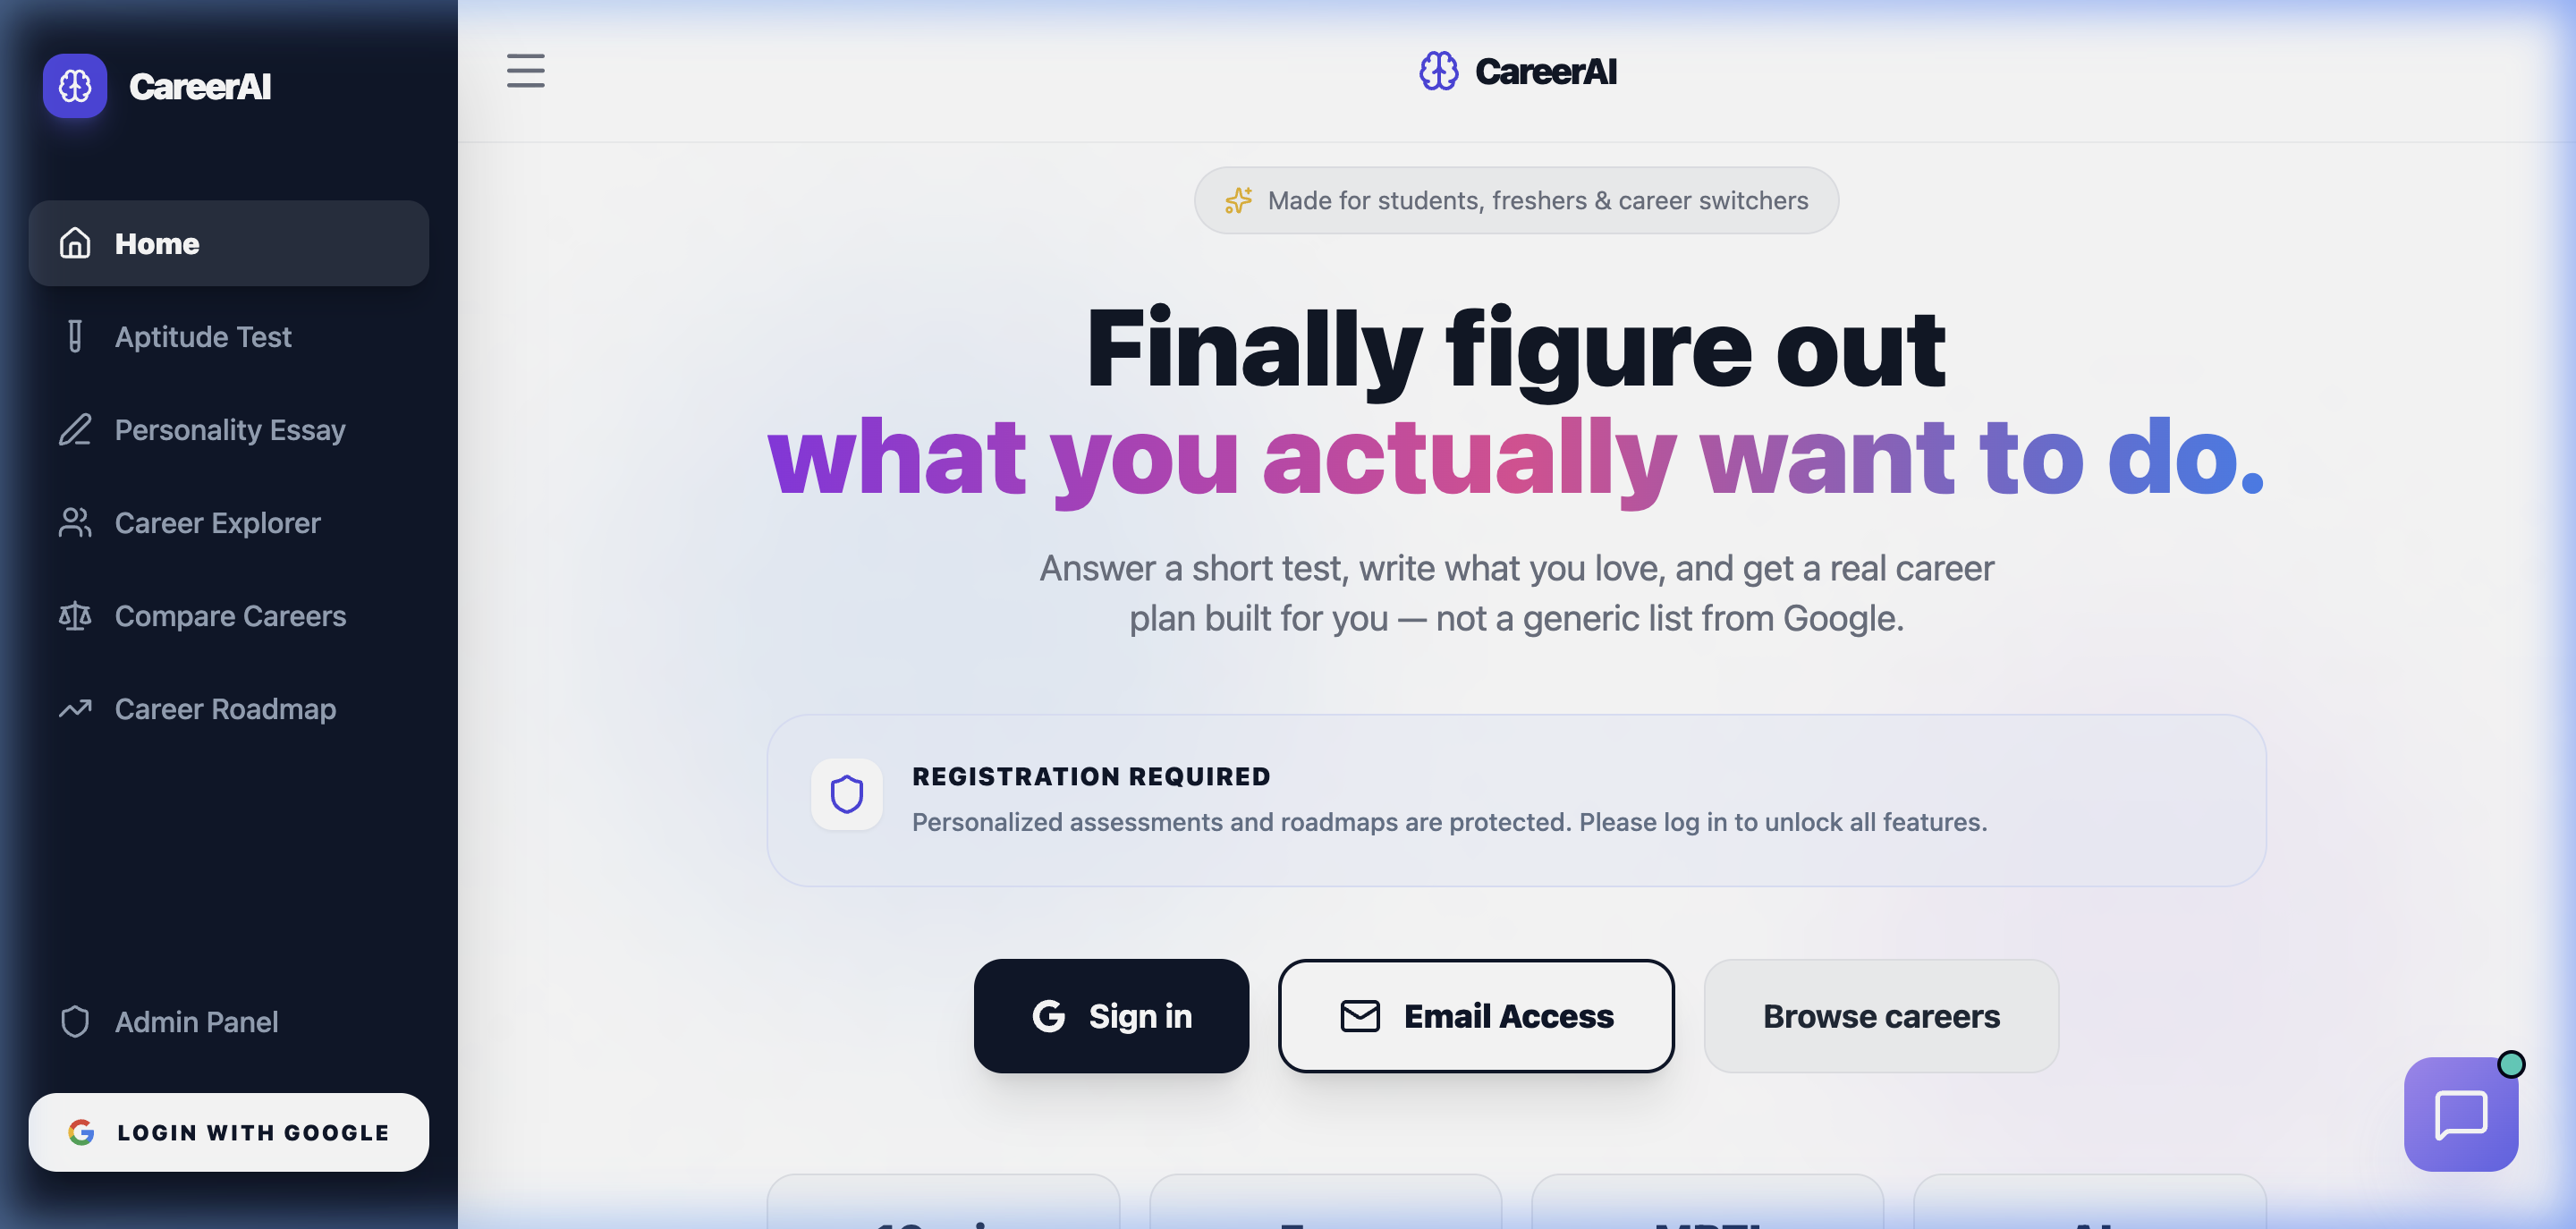
\includegraphics[width=0.9\textwidth]{project/images/home.png}
\caption{Landing Page of AI Powered Career Counselling System}
\label{fig:home}
\end{figure}

\begin{figure}[H]
\centering
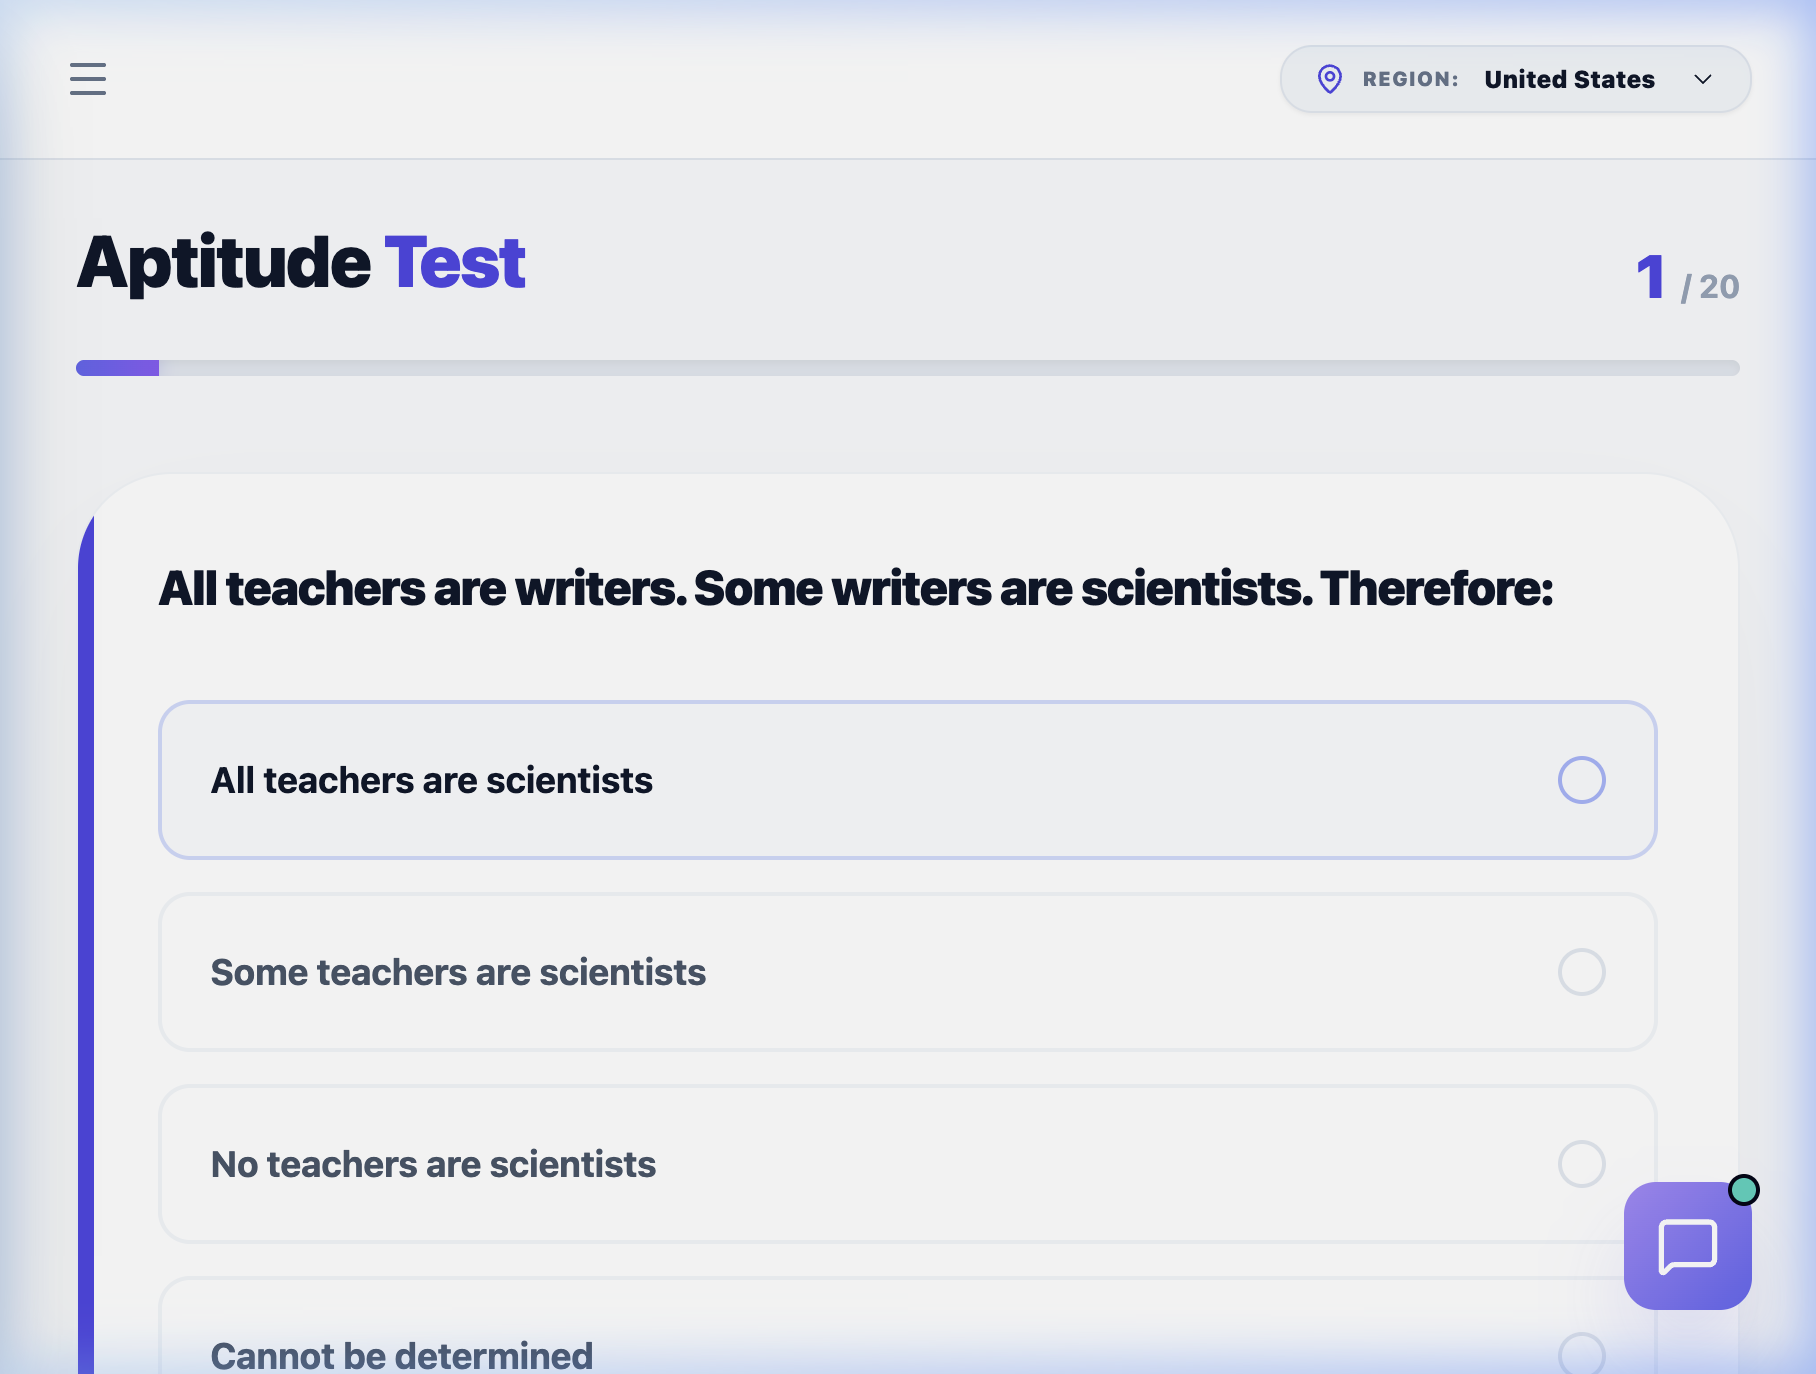
\includegraphics[width=0.9\textwidth]{project/images/how_it_works.png}
\caption{Assessment Introduction and Logic Overview}
\label{fig:how}
\end{figure}

\begin{figure}[H]
\centering

\includegraphics[width=0.9\textwidth]{project/images/login.png}
\caption{Secure User Authentication via Google OAuth 2.0}
\label{fig:login}
\end{figure}

\begin{figure}[H]
\centering
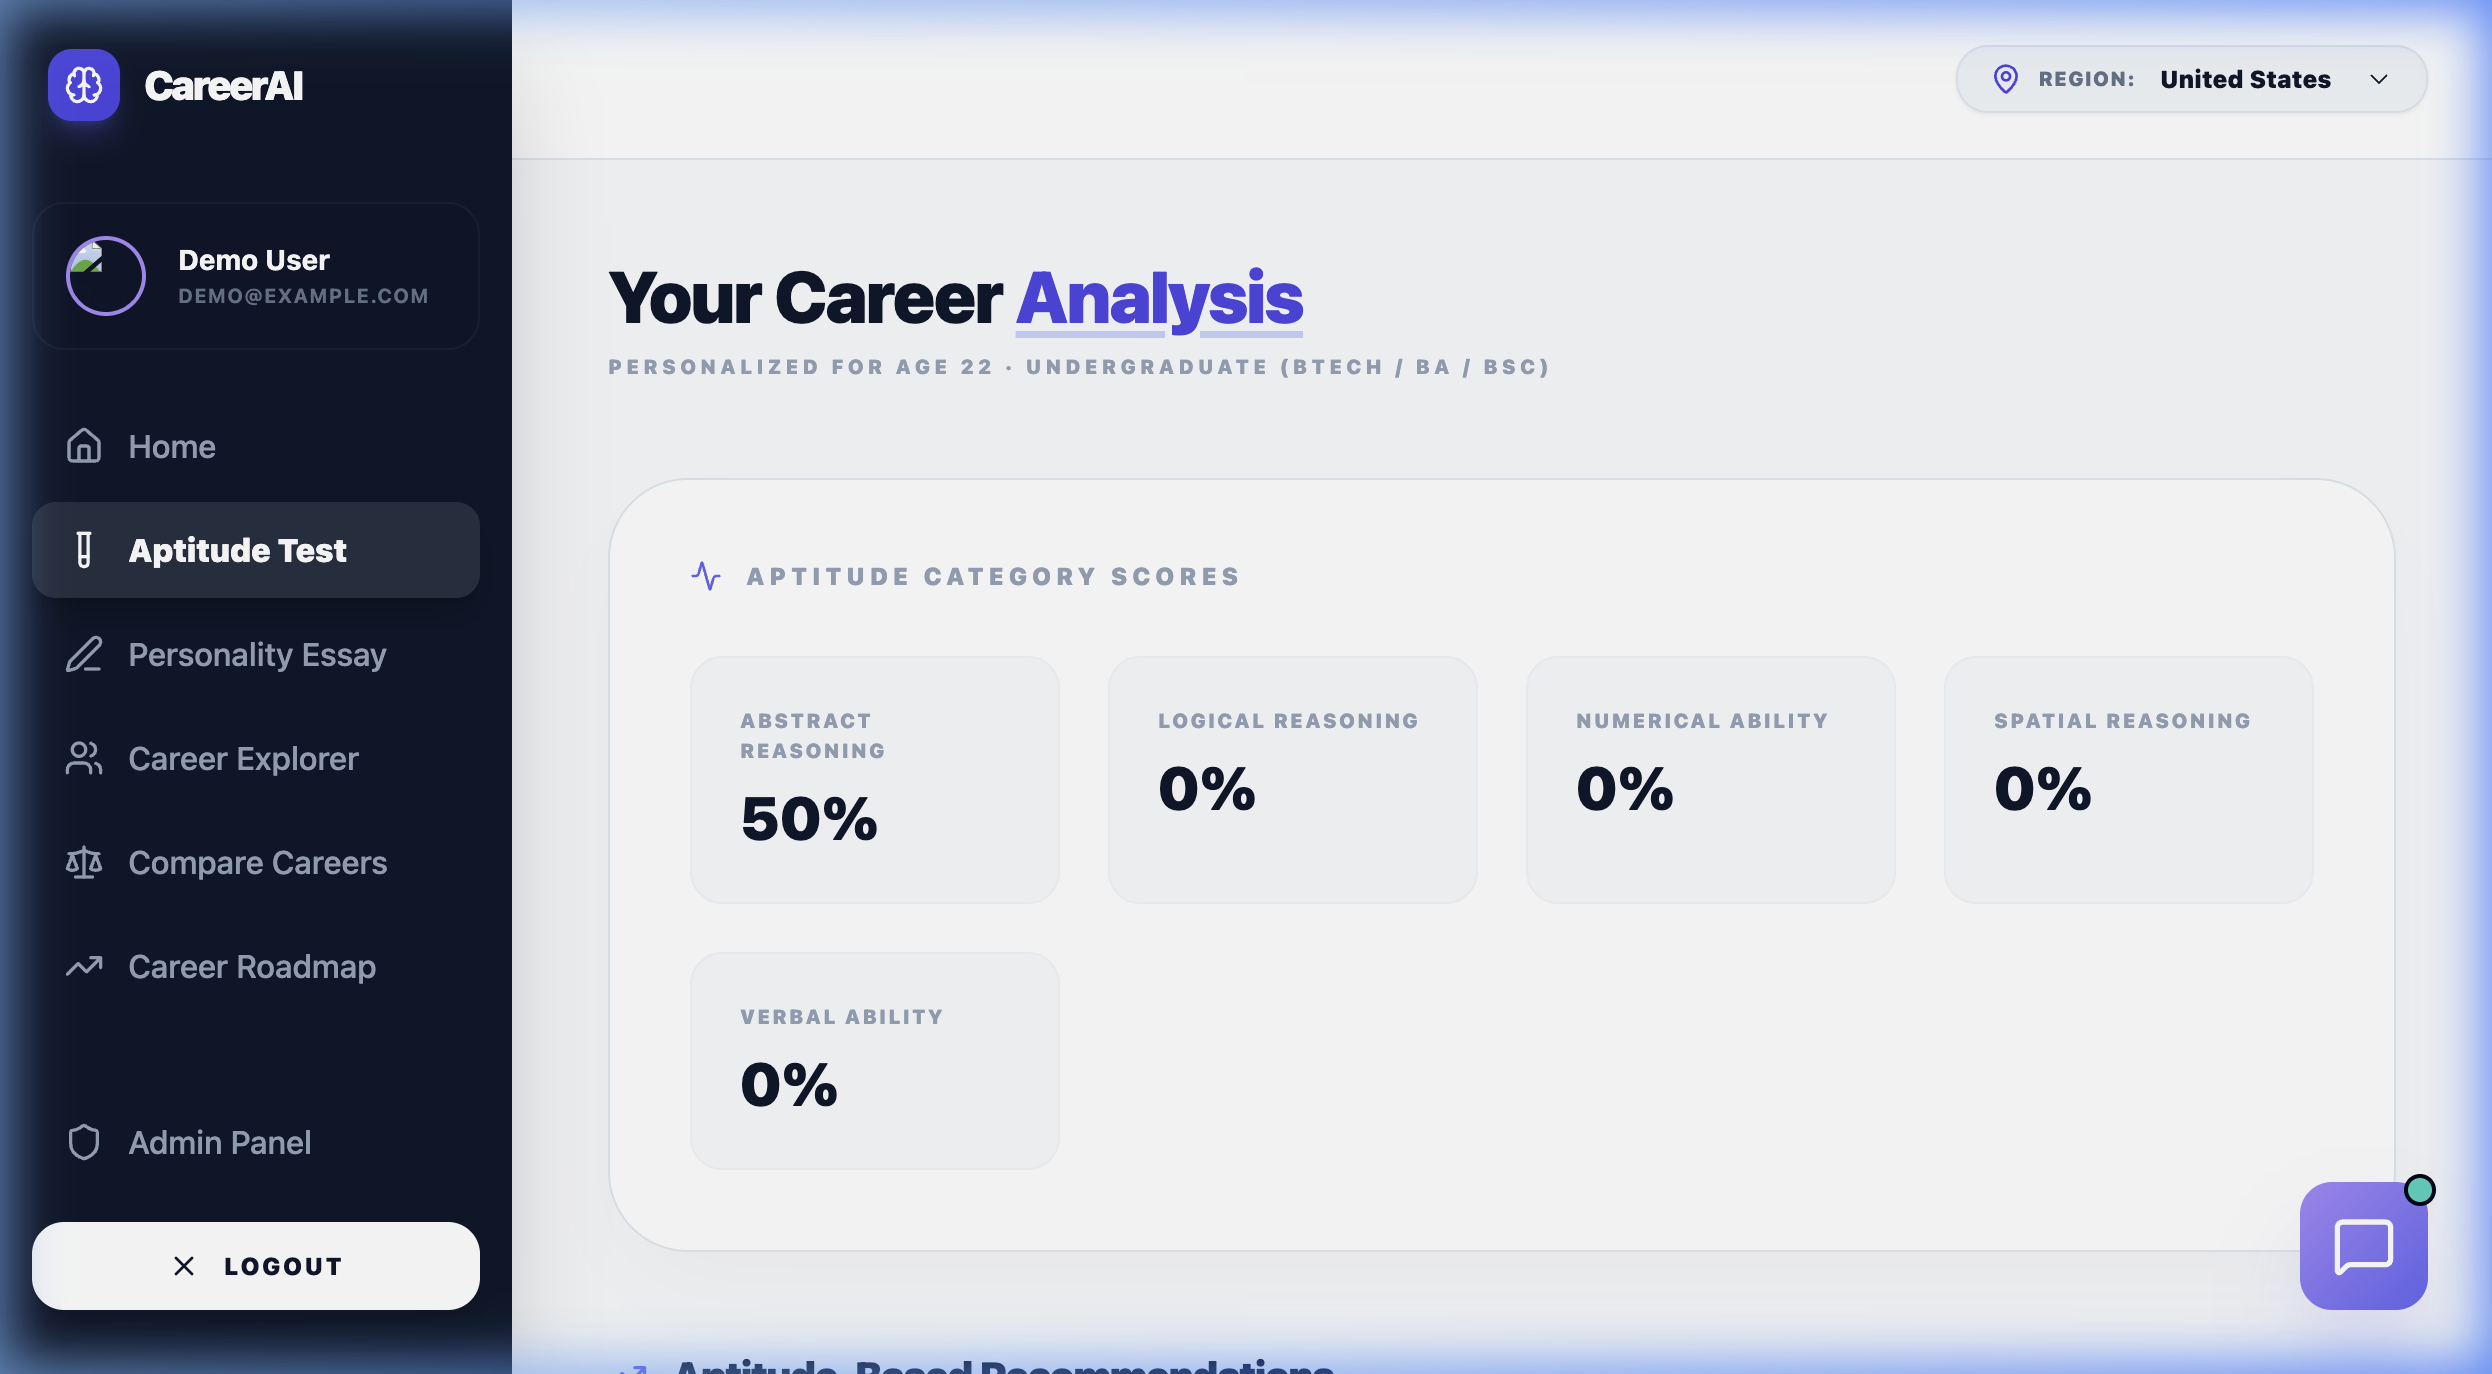
\includegraphics[width=0.9\textwidth]{project/images/dashboard.png}
\caption{Interactive Career Recommendation Dashboard}
\label{fig:dashboard}
\end{figure}

\begin{figure}[H]
\centering
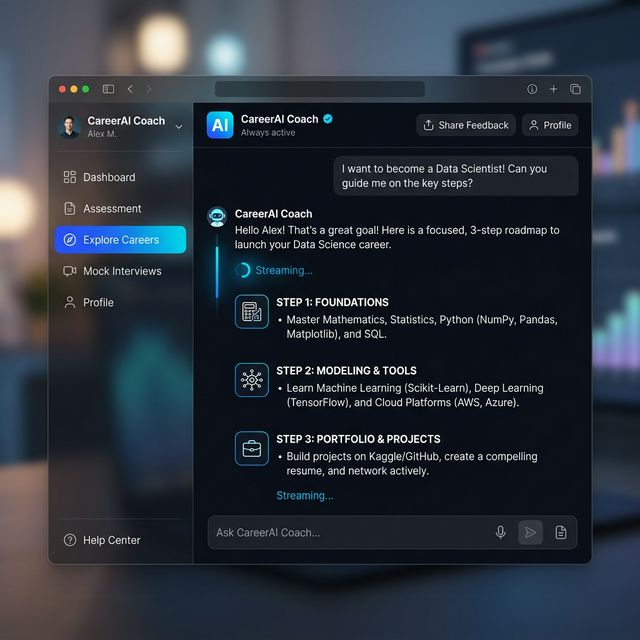
\includegraphics[width=0.9\textwidth]{project/images/contact.png}
\caption{AI Career Coach Chatbot for Real-time Guidance}
\label{fig:contact}
\end{figure}

\vspace{-1cm}
\chapter{Conclusion and Future Scope}
\section{Conclusion}
\paragraph{}The AI Powered Career Counselling System (CareerAI) has been developed to address the significant communication and guidance gap between students and expert career advisors. The system uses modern technologies such as Computerized Adaptive Testing (CAT), Natural Language Processing (NLP), and Large Language Models (LLMs) to recognize a user's cognitive strengths and career aspirations, converting them into actionable roadmaps and personalized guidance in real-time.

The project demonstrates that intelligent career counseling can be successfully implemented using a web-based, AI-driven approach. It provides a premium and user-friendly interface that allows students to assess their skills and receive immediate technical feedback. This helps improve career alignment in various environments such as high schools, colleges, and professional development centers.

Although the system performs well for a wide range of career domains, its accuracy ultimately depends on factors like the honesty of user responses and the underlying reasoning capabilities of the Gemini model. Despite these limitations, the project proves to be a powerful and practical solution for enhancing educational accessibility and promoting data-driven career growth for the youth.

\section{Future Scope}
{}The future scope of the AI Powered Career Counselling System is significant, as the current system can be further enhanced to improve its precision, cultural relevance, and long-term utility. One of the major improvements can be the expansion of the career database to include 100+ specialized vocational paths, allowing the system to support more niche industry guidance and detailed skill-gap analysis.
\begin{itemize}
 \item The accuracy of the recommendation engine can be improved by using fine-tuned models on specific educational datasets and larger user feedback loops. This will help the system provide more nuanced advice across different geographical markets and shifting job trends. The integration of real-time LinkedIn or Job Board connectivity can also be added so that recognized roadmaps can be converted into actual job applications, making the career transition more direct and efficient.
 \item The system can be further developed into a cross-platform mobile application, making it more portable and accessible for everyday career tracking. Real-time mentorship integration can also be implemented to connect students directly with human experts once the AI has mapped their initial path. Additionally, support for multiple regional languages (such as Hindi or Spanish) can be added so that the recommendations can reach students who are not proficient in English.
 \item In the future, the system can also be integrated with Virtual Reality (VR) modules to provide "Day-in-the-Life" experiences for different careers, allowing students to virtually experience a profession before committing to it. These enhancements will make the system more immersive, user-friendly, and widely applicable, contributing to better workforce planning and individual fulfillment on a global scale.
\end{itemize}

\chapter{UN Sustainable Development Goals}

\section{Mapping with UN Sustainable Development Goals}

\paragraph{}
The United Nations has defined 17 Sustainable Development Goals (SDGs) to address global challenges such as poverty, inequality, education, and social inclusion. These goals aim to achieve a better and more sustainable future for all by the year 2030.

\paragraph{}
The AI Powered Career Counselling System (CareerAI) is mainly aligned with \textbf{SDG 4: Quality Education}, \textbf{SDG 8: Decent Work}, and \textbf{SDG 10: Reduced Inequalities}. The project focuses on improving access to high-quality vocational guidance for all students, thereby promoting inclusive learning and reducing the information barriers that lead to career mismatch.

\paragraph{}
The system helps individuals with diverse cognitive strengths to better understand and interact with the modern job market, which contributes to equal opportunities in education and long-term economic participation.

\begin{table}[H]
\centering
\caption{SDG Mapping for CareerAI}
\begin{tabular}{|l|p{6cm}|p{8cm}|}
\hline
\multicolumn{3}{|l|}{\textbf{SDG Title : Quality Education (SDG 4), Decent Work (SDG 8) and Reduced Inequalities (SDG 10)}} \\
\hline
\textbf {S.No} & \textbf{Objective} & \textbf{Outcome}\\
\hline

1 & Provide inclusive and accessible career guidance for all students 
& The system enables democratized access to expert-level counseling, improving decision-making for learners from all backgrounds. \\

\hline

2 & Reduce the skills gap between education and industry 
& Targeted 12-month roadmaps help individuals acquire specific skills needed for sustainable, decent work. \\

\hline

3 & Promote the use of AI for personalized and lifelong learning 
& The system integrates LLMs and adaptive testing to support a smart, evolving guidance environment. \\

\hline

4 & Reduce socio-economic inequalities in career outcomes 
& The project helps in reducing inequalities by providing high-end counseling to students who cannot afford private human counselors. \\

\hline

\end{tabular}

\label{tab:merged}
\end{table}

\vspace{-1cm}
\input{project/References.tex}
\input{project/ProjectPoster.tex}
\vspace{-1cm}
\begin{center}
\LARGE{\textbf{CERTIFICATE}}
\end{center}

\vspace{1cm}
\large
This is to certify that \textbf{Mr. Sanyam Jain} and \textbf{Ms. Tanisha Aggarwal}, students of B.Tech (Computer Science \& Engineering (DS)) 8th semester, have submitted their Project Report entitled \textbf{"AI POWERED CAREER COUNSELLING SYSTEM"} under my guidance.

\vspace{3cm}
\begin{table}[h]
\centering
\begin{tabular}{p{5cm}p{5cm}}
\dotfill & \dotfill \\
\textbf{Ms. Mani Butwall} & \textbf{Mr. Sumit Kumar} \\
Assistant Professor & Assistant Professor \\
(Mentor) & (Coordinator) \\
\end{tabular}
\end{table}

\vspace{2cm}
\noindent
\textbf{Department of Computer Science and Engineering (DS)} \\
Swami Keshvanand Institute of Technology, Jaipur
\clearpage

\vspace{-1cm}
\input{project/Githublink.tex}
\end{document}
